\section{The balanced puncture observable}\label{c01-c1-the-balanced-puncture-observable}

A contraction of the two vacua will count polygons separating two specified cylinder faces. We first establish that positive interpretation and then the interpolation data that characterize the contraction.

Divide the ordered sites into a first block A of size \(n\) and remaining block B of size \(m=N-n\). Define
\[
 X_{n,m}(X;\kappa)=\Omega(X^{-1})^t D_{\kappa/\zeta}^{\rm A}\,\Omega(X)
\]
where the diagonal multiplies by \((\kappa/\zeta)^{\sum_{j\in{\rm A}}h_j}\), for \(\kappa\ne0\).
\begin{samepage}
\begin{proposition}[Physical separator pairing]\label{prop:pv:physical-pairing}
For two homogeneous blocks of equal size $n$,
\[
 X_{n,n}(1,\ldots,1;\kappa)=F_n(\kappa+\kappa^{-1}).
\]
Here the left side is the bilinear vacuum contraction just defined and the right side is the positive polygon polynomial from Section~\ref{sec:pv:introduction}.
\end{proposition}
\end{samepage}

\begin{proof}
Work first at finite height with homogeneous sites. If \(|0\rangle\)
is the empty tensor, the lower and upper boundary states are
\[
 |u_H\rangle=\mathcal T_\zeta(t)^H|0\rangle,
 \qquad
 \langle v_H|=\langle0|\mathcal T_{\zeta^{-1}}(t)^H.
\]
Every empty-to-empty entry is 1 by loop cancellation.
Lemma~\ref{lem:pv:physical-eigenline} and the normalized left and right
eigenvectors therefore give
\[
 |u_H\rangle\longrightarrow\Omega(1,\ldots,1),\qquad
 \langle v_H|\longrightarrow\Omega(1,\ldots,1)^t.
\]
The upper state is obtained by rows between the gluing cut and an empty
upper boundary; its twist is \(\zeta^{-1}\). This identifies the
reciprocal left eigenvector geometrically by the rank-one limit.
At nonsingular physical data we always use these analytic states,
including when their rational formulas are evaluated by a limit.

The finite contraction \(\langle v_H|D_{\kappa/\zeta}^{\rm A}|u_H\rangle\)
glues matching occupied ports to make disjoint polygons. Internal gauge
factors telescope under this gluing. It has three
directed seams: from the lower boundary to \(f\), with weight
\(\zeta\); from \(f\) to the upper boundary, with weight
\(\zeta^{-1}\); and from the block-division face \(f'\) to \(f\)
along block A, with weight \(\kappa/\zeta\). See
Figure~\ref{fig:pv:seams}. Positive crossing is toward the left of a
directed seam. For an oriented simple polygon, let \(L(a)\) indicate
whether \(a\) lies on its left. The signed crossing number of a seam
\(a\to b\) is \(L(a)-L(b)\), so its three seam factors multiply to
\[
 \zeta^{L(-\infty)-L(f)}
 \zeta^{-L(f)+L(+\infty)}
 (\kappa/\zeta)^{L(f')-L(f)}.
\]
Here the two end indicators may be taken at the empty finite boundaries.
For a contractible polygon oriented with interior left, the turn factor
is \(i=\zeta\) and both end indicators are zero. For an essential
polygon oriented with upper end left, the turn factor is 1 and the
end indicators are zero and one. In both cases the total factor is
\[
 \zeta^{1-L(f)-L(f')}\kappa^{L(f')-L(f)}.
\]
The reverse orientation contributes its inverse. Equal indicators
therefore give \(\zeta+\zeta^{-1}=0\), whereas unequal indicators
give \(\eta=\kappa+\kappa^{-1}\). Exactly the separating polygons
survive, with their critical vertex weights.

At each finite height the contraction is consequently a polynomial
in \(\eta\) with nonnegative coefficients. Its degree is at most
\(n\), since every separating polygon uses a distinct port of block A.
The coefficients increase as the height grows. At any fixed positive
\(\eta\), convergence of the two boundary states bounds the
contractions, and hence bounds every coefficient. Their finite limits
are exactly the infinite-cylinder polygon sums. Passing to the limit
coefficientwise proves the claimed identity for every \(\kappa\ne0\).

\end{proof}

\begin{figure}[tb]
\centering
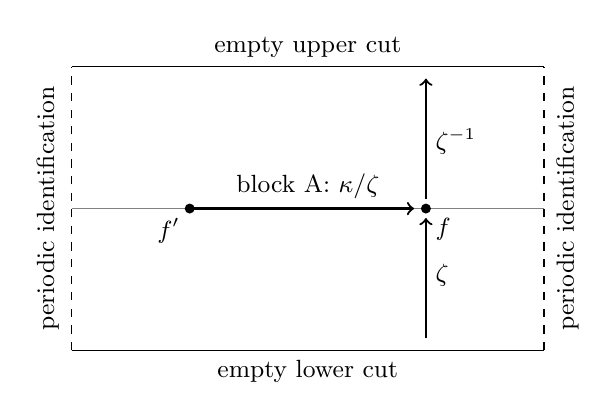
\begin{tikzpicture}[x=1cm,y=1cm,every node/.style={font=\small}]
 \draw[dashed] (-3,-1.8)--(-3,1.8);
 \draw[dashed] (3,-1.8)--(3,1.8);
 \draw (-3,-1.8)--(3,-1.8);
 \draw (-3,1.8)--(3,1.8);
 \draw[gray] (-3,0)--(3,0);
 \draw[thick,->] (1.5,-1.65)--(1.5,-.12);
 \draw[thick,->] (1.5,.12)--(1.5,1.65);
 \draw[thick,->] (-1.5,0)--(1.35,0);
 \fill (1.5,0) circle (1.8pt);
 \fill (-1.5,0) circle (1.8pt);
 \node[below right] at (1.5,0) {$f$};
 \node[below left] at (-1.5,0) {$f'$};
 \node[right] at (1.5,-.85) {$\zeta$};
 \node[right] at (1.5,.85) {$\zeta^{-1}$};
 \node[above] at (0,0) {block A: $\kappa/\zeta$};
 \node[above] at (0,1.8) {empty upper cut};
 \node[below] at (0,-1.8) {empty lower cut};
 \node[rotate=90] at (-3.3,0) {periodic identification};
 \node[rotate=90] at (3.3,0) {periodic identification};
\end{tikzpicture}
\caption{The finite cylinder, cut open along the two identified dashed
sides. The middle line is the gluing cut; the arrows are directed twist
seams, not polygon segments. Block A follows the site order from $f$
toward $f'$, while its seam is directed from $f'$ to $f$. The empty
upper and lower cuts recede to the cylinder ends in the limit.}
\label{fig:pv:seams}
\end{figure}

\begin{remark}[Comparison of the scalar and physical pairings]\label{rem:pv:scalar-comparison}
For $N=2n$, reversing both the numerator and Vandermonde conventions
leaves the empty polynomial unchanged:
\[
 S_{2n}(X)=\prod_{i<j}\frac{D(x_i,x_j)}{x_j-x_i}
 \operatorname{Pf}\!\left[\frac{x_j^2-x_i^2}{D(x_i,x_j)}\right].
\]
The prefactor changes by $(-1)^{n(2n-1)}$ and the Pfaffian by
$(-1)^n$, whose product is one. This is exactly the scalar convention
of~\cite[Section~5.2]{DiskTransfer2026}.

Multiplying our lattice coordinates by $\sqrt3$ gives honeycomb edge
length one. It preserves polygon vertices, critical weights, and which
polygons separate the marks, and therefore preserves $F_n$ on the
rescaled cylinder.
For $n\ge3$, the disk construction in
\cite[Section~5.3]{DiskTransfer2026} identifies its physical pairing
with this same polygon sum. These comparisons concern the scalar
polynomial and the physical observable; the inhomogeneous vectors and
their denominator estimates remain separate constructions.
\end{remark}

\subsection{Interpolation of the contraction}

The following characterization will identify the finite color formula
in Section~\ref{c01-c1-color-formula-and-small-cycle-gas}. It applies
at generic parameters; it does not assert that \(S_N\) is nonzero
at every complex specialization. In the displays below we separate
the site lists of the two blocks by a semicolon.

\begin{proposition}[Interpolation of the pairing]\label{prop:pv:pairing-interpolation}
Fix \(\kappa\ne0\) and put \(\eta=\kappa+\kappa^{-1}\).
The family \(X_{n,m}\) is uniquely determined among rational functions
by the following properties. It is symmetric separately in its two
blocks, and \(S_N^2X_{n,m}\) is polynomial of degree at most
\(2(N-1)\) in each site, where \(N=n+m\). Within block A its
reductions are
\[
\begin{aligned}
 X_{n,m}(a,Ta,A';B)&=X_{n-2,m}(A';B),\\
 X_{n,m}(a,t^2a,A';B)&=X_{n-1,m}(ta,A';B),\\
 \lim_{a\to0\text{ or }\infty}X_{n,m}(a,A';B)
 &=X_{n-1,m}(A';B),
\end{aligned}
\]
The pair reductions require \(n\ge2\), and the extreme reduction
requires \(n\ge1\); the analogous rules hold in block B with \(m\)
in place of \(n\). The initial value is
\(X_{0,0}=1\), and at every balanced size \(n=m>0\),
\[
 X_{n,n}(a_1,\ldots,a_n;Ta_n,\ldots,Ta_1)=(1+\eta)^n.
\]
\end{proposition}

\begin{proof}
Separate block symmetry follows from exchange and its inverse,
transpose symmetry of \(F\), and charge conservation. Reciprocity
of \(S_N\) shows that \(S_N^2X_{n,m}\) is the contraction of two
polynomial vectors, each of degree at most \(N-1\) per site; this
gives the degree bound.

For the extreme reductions, the complementary vanishing of nonzero
spins on the two sides leaves only the spin-zero limit in
Corollary~\ref{cor:pv:normalized-reductions}. At an adjacent cup the
right vector inserts \(C\). In the reciprocal vector, the projection
onto the same channel inserts \(C/r_0(T)\): exchanging its reversed
pair into cup order acts by \(F(T)=r_0(T)P_0\). Contraction cancels
the scalar because \(C^tC=r_0(T)=-n_0\), and the block twist
preserves the pair. At the other fusion, use
\(F(t^2)=n_0P_1\) and \(I^tI=n_0\,1\) in the same way.
The block twist on the image of \(I\) is the single-site twist.
These are rational identities on the generic domain.

At the balanced specialization, successive nested cups in the right
vector force spins \(h\) on A with opposite mates in B and amplitudes
\(\prod q^{5h}\). Rotate B to the beginning in the reciprocal vector.
Its cups now face the other way, so in the original order its amplitudes
are \(\prod\zeta^h q^{-5h}\). Together with the block insertion,
each pair contributes \(\sum_{h=0,\pm1}\kappa^h=1+\eta\).
This gives the last specialization.

For uniqueness, suppose two families agree at smaller sizes, and let
\(A(X)\) be their difference at \((n,m)\), multiplied by \(S_N^2\).
The zero and infinity reductions give respectively
\(x_i\mid A\) and \(\deg_{x_i}A\le2N-3\) at each site. The
cup and second fusion, in both orders, give four factors for each
intra-block pair. Thus
\[
 Q(X)=\left(\prod_{i=1}^Nx_i\right)
 \prod_{P\in\{\mathrm A,\mathrm B\}}
 \prod_{\substack{i<j\\i,j\in P}}
 \prod_{d\in\{2,3,5,6\}}(x_j-t^d x_i)
 \quad\hbox{divides }A(X).
\]
In a site of A this divisor has degree \(4(n-1)+1\), leaving
\[
 \deg_{x_i}(A/Q)\le2N-3-[4(n-1)+1]=2(m-n).
\]
In a site of B the remaining degree is at most \(2(n-m)\).
An unbalanced difference is therefore zero. In a balanced case the
quotient is a scalar; the nested-cup specialization fixes it to zero,
since it is generically off the zero sets of both \(Q\) and \(S_N\).
Induction from \(X_{0,0}=1\) completes uniqueness.
\end{proof}
